\documentclass[a4paper,12pt]{article}

%% Definitioner för vågfysikrapporten-dokument

%% Text-kodning, språk samt PS-font
\usepackage[utf8]{inputenc}
\usepackage[T1]{fontenc}
\usepackage{ae,aecompl}
\usepackage{listings}
% % bitmap-grafik
\usepackage{graphicx}
% % matematik
\usepackage{amsmath}
\usepackage{mathtools}
\usepackage{latexsym}
\usepackage{graphicx}

%% Paragrafformat
\setlength{\parindent}{0pt}
\setlength{\parskip}{1ex plus 0.5ex minus 0.2ex}

%% Format för datum
\newcommand{\twodigit}[1]{\ifthenelse{#1<10}{0}{}{#1}}
\newcommand{\dagensdatum}{
\number\year-\twodigit{\number\month}-\twodigit{\number\day}}

%% Sidhuvud och sidfot
\usepackage{fancyhdr}
\pagestyle{fancy}
\lhead{Alexander Poole}
\chead{INLÄMNINGSUPPGIFT 1-1080}
\rhead{TSEA05}
\lfoot{alepo020@student.liu.se}
\cfoot{{\ } \\ \thepage}
\rfoot{19920829-0057}

%%Title
\title{TSEA05 \\ INLÄMNINGSUPPGIFT 1-1080}
\author{Alexander Poole}

%%Gray box
\usepackage{mdframed}





%%Dokumentets början
\begin{document}
\maketitle
\thispagestyle{empty}
\newpage

%%TODO
\section*{Problemformulering}
Målet med uppgiften är att ta det givna enborten A-B i figur \ref{fig:original} och förenkla det till dess Theveninekvivalenta eller Nortonekvivalenta motsvarighet, se figur \fig{}. För att åstakomma detta får Ohms lag, KCL, KVL samt slinganalys, nodanalys eller metoden med incidensmatriser användas.

\section*{Lösning}
Problemet löses med hjälp av slinganalys.

\begin{figure}[h]
\centering
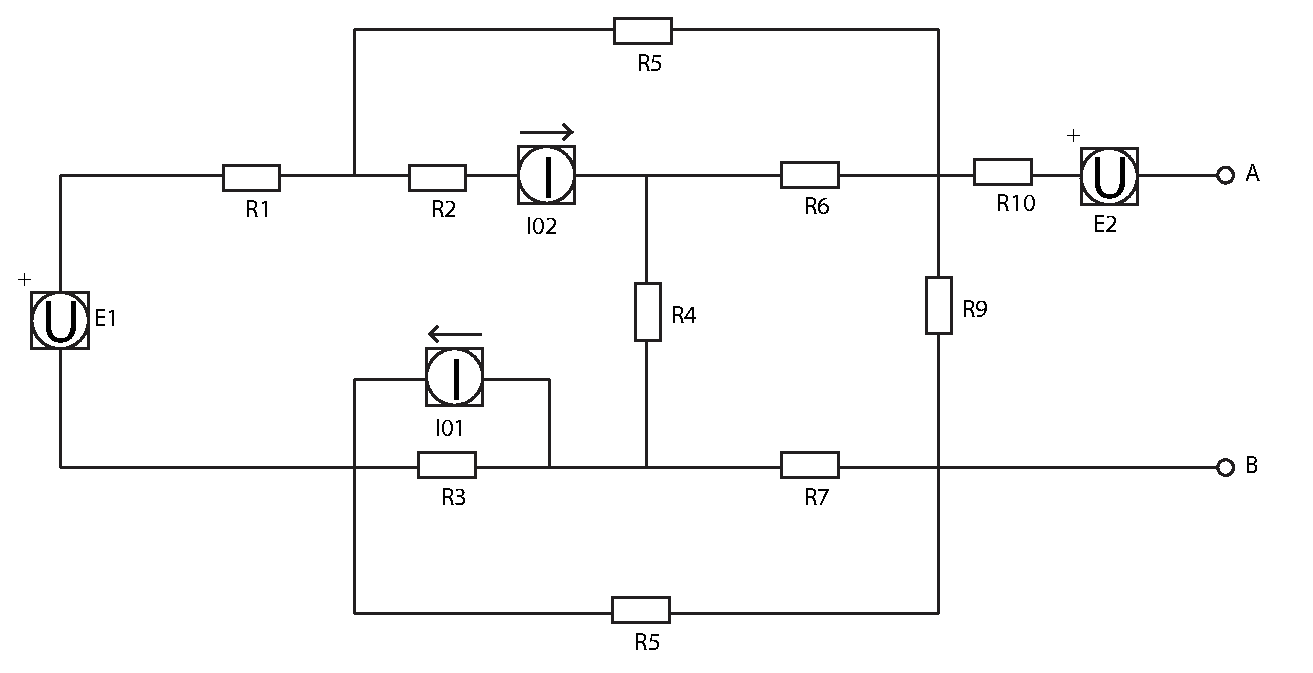
\includegraphics[width=1\textwidth]{bilder/originalnat.eps}
\caption{Nät givet i uppgiften.}
\label{fig:original}
\end{figure}

Föränklar bort R2 ty i serie med strömkällan I02. Förenklar bort den ensamma strömkällan I02. Sätter in strömmar i de slingor som uppstår, se \fig{fig:modnat}.

\begin{figure}[h]
\centering
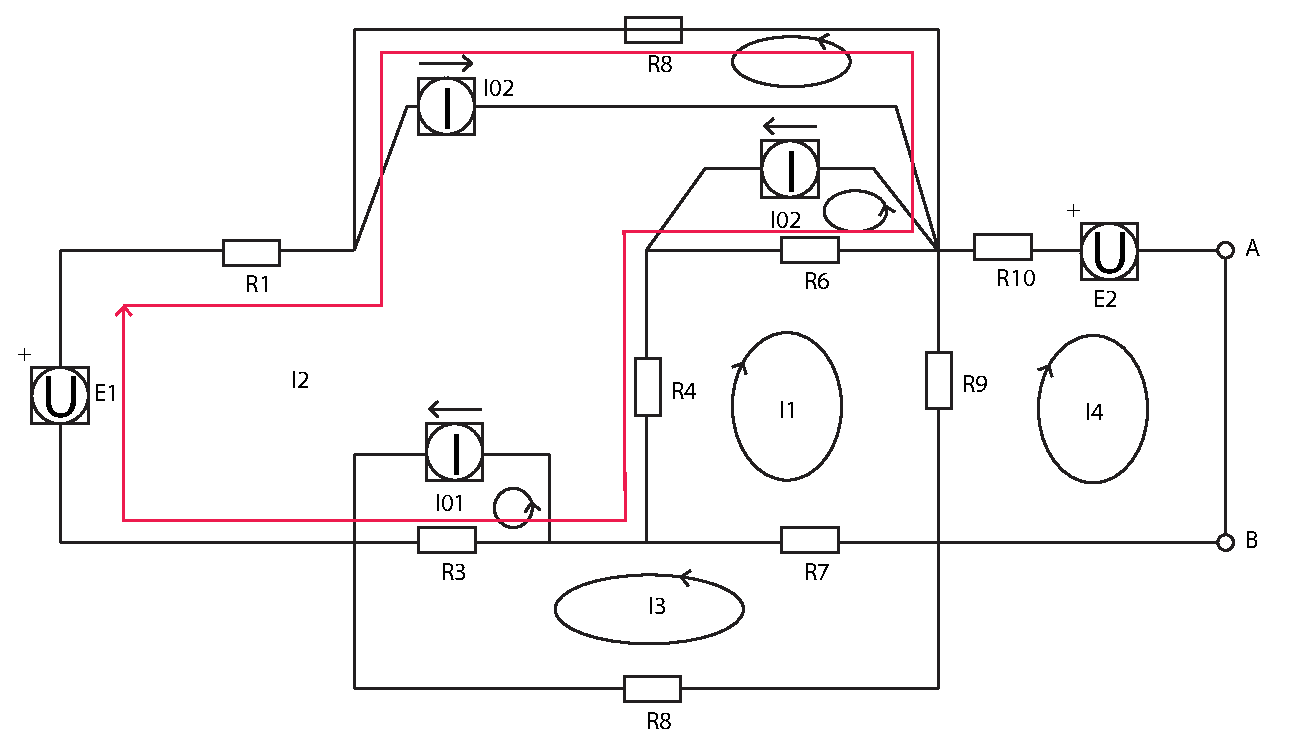
\includegraphics[width=1\textwidth]{bilder/modnat.eps}
\caption{Nät efter förenklingar, med angivna slingor och strömmar.}
\label{fig:modnat}
\end{figure}

KVL annvänds på samtliga slingor detta ger ekvation \ref{ekv:KVLrough}

\begin{equation}
V=\sqrt{0.159g\lambda+6.2\frac{\gamma}{\rho\lambda}}
\label{ekv:KVLrough}
\end{equation}

\end{document}


